\documentclass[a4paper,landscape,11pt]{article}

\usepackage{kpfonts}
\usepackage{inconsolata}
\usepackage{listings}
\usepackage{color}

\usepackage[brazilian]{babel}
\usepackage[utf8]{inputenc}
\usepackage[T1]{fontenc}

\usepackage[tocflat]{tocstyle}
\usetocstyle{standard}

\usepackage{natbib}
\usepackage{url}
\usepackage{amsmath}
\usepackage{graphicx}
\graphicspath{{images/}}
\usepackage{parskip}
\usepackage{fancyhdr}
\usepackage{vmargin}
\setmarginsrb{3 cm}{2.5 cm}{3 cm}{2.5 cm}{1 cm}{1.5 cm}{1 cm}{1.5 cm}

\title{Método de Gauss-Seidel}			                    		% Title
\author{Renato Pontes\\Mateus Ildefonso}	% Author
\date{11 de Dezembro de 2016}										% Date

\makeatletter
\let\thetitle\@title
\let\theauthor\@author
\let\thedate\@date
\makeatother

\pagestyle{fancy}
\fancyhf{}
\rhead{\theauthor}
\lhead{\thetitle}
\cfoot{\thepage}

\usepackage{hyperref}
\hypersetup{colorlinks=true,allcolors=blue}
\usepackage{hypcap}
\begin{document}
\lstset{basicstyle=\footnotesize\ttfamily,breaklines=true, tabsize=4}
%%%%%%%%%%%%%%%%%%%%%%%%%%%%%%%%%%%%%%%%%%%%%%%%%%%%%%%%%%%%%%%%%%%%%%%%%%%%%%%%%%%%%%%%%

\begin{titlepage}
	\centering
    \vspace*{0.5 cm}
    
\includegraphics[scale = 0.50]{minerva.jpg}\\[1.0 cm]	% University Logo
    \textsc{\LARGE Universidade Federal do Rio de Janeiro}\\[2.0 cm]
                                                        % University Name
	\textsc{\Large MAB528}\\[0.5 cm]				    % Course Code
	\textsc{\large Tópicos Especiais em Algoritmos}\\[0.5 cm]	% Course Name
	\rule{\linewidth}{0.2 mm} \\[0.4 cm]
	{ \huge \bfseries \thetitle}\\
	\rule{\linewidth}{0.2 mm} \\[1.5 cm]
	
	\begin{minipage}{0.4\textwidth}
		\begin{flushleft} \large
			\emph{Aluno:}\\
			\theauthor
			\end{flushleft}
			\end{minipage}~
			\begin{minipage}{0.4\textwidth}
			\begin{flushright} \large
			\emph{DRE:} \\
			113131049\\114073032					% Your Student Number
		\end{flushright}
	\end{minipage}\\[2 cm]
	
	{\large \thedate}\\[2 cm]
 
	\vfill
	
\end{titlepage}

%%%%%%%%%%%%%%%%%%%%%%%%%%%%%%%%%%%%%%%%%%%%%%%%%%%%%%%%%%%%%%%%%%%%%%%%%%%%%%%%%%%%%%%%%

\tableofcontents
\pagebreak

%%%%%%%%%%%%%%%%%%%%%%%%%%%%%%%%%%%%%%%%%%%%%%%%%%%%%%%%%%%%%%%%%%%%%%%%%%%%%%%%%%%%%%%%%

\section{Documentação da solução}

\subsection*{Ambiente}
A aplicação foi desenvolvida no \textit{Windows}. Seguem as especificações da GPU utilizada para testes:

\begin{lstlisting}
Device 0: "GeForce GT625M"
  CUDA Driver Version / Runtime Version          8.0 / 7.5
  CUDA Capability Major/Minor version number:    2.1
  Total amount of global memory:                 1024 MBytes (1073741824 bytes)
  ( 2) Multiprocessors x ( 48) CUDA Cores/MP:    96 CUDA Cores
  GPU Clock rate:                                1250 MHz (1.25 GHz)
  Memory Clock rate:                             900 Mhz
  Memory Bus Width:                              64-bit
  L2 Cache Size:                                 131072 bytes
  Max Texture Dimension Size (x,y,z)             1D=(65536), 2D=(65536,65535), 3D=(2048,2048,2048)
  Max Layered Texture Size (dim) x layers        1D=(16384) x 2048, 2D=(16384,16384) x 2048
  Total amount of constant memory:               65536 bytes
  Total amount of shared memory per block:       49152 bytes
  Total number of registers available per block: 32768
  Warp size:                                     32
  Maximum number of threads per multiprocessor:  1536
  Maximum number of threads per block:           1024
  Maximum sizes of each dimension of a block:    1024 x 1024 x 64
  Maximum sizes of each dimension of a grid:     65535 x 65535 x 65535
  Maximum memory pitch:                          2147483647 bytes
  Texture alignment:                             512 bytes
  Concurrent copy and kernel execution:          Yes with 1 copy engine(s)
  Run time limit on kernels:                     Yes
  Integrated GPU sharing Host Memory:            No
  Support host page-locked memory mapping:       Yes
  Alignment requirement for Surfaces:            Yes
  Device has ECC support:                        Disabled
  Device supports Unified Addressing (UVA):      Yes
  Device PCI Bus ID / PCI location ID:           2 / 0
  Compute Mode:
     < Default (multiple host threads can use ::cudaSetDevice() with device simultaneously) >

deviceQuery, CUDA Driver = CUDART, CUDA Driver Version = 8.0, CUDA Runtime Version = 7.5, NumDevs = 1, Device0 = GeForce GT625M
\end{lstlisting}

Estas informações foram extraídas a partir do executável \texttt{deviceQuery}, disponível como código de exemplo na plataforma CUDA.

Descrevemos a seguir cada um dos módulos do programa. Em qualquer referência a caminhos de arquivos assumimos que estamos no diretório raiz \texttt{gauss\_seidel}.

\subsection{main.c}
O arquivo \texttt{main.c} é responsável pela alocação de memória da matriz que representa a malha e também pela definição dos parâmetros globais do problema, utilizando variáveis globais (tais como $N_1,N_2,h_1,h_2,\omega$, etc). Foram guardados na memória apenas os pontos que não são conhecidos. As bordas foram guardadas em variáveis comuns. Por esse motivo, os valores da matriz devem ser recuperados por meio de uma função(\texttt{float get\_v(int, int)}), que lida com os índices inválidos das bordas.

Além disso, ela também valida os argumentos passados pela linha de comando e escolhe que método deve ser executado. O método de Gauss-Seidel foi implementado nas duas formas descritas no enunciado, cada uma delas com uma versão sequencial e outra paralela.

A aplicação executa apenas uma versão do método a cada execução. Para comparar os tempos de execução entre uma versão e outra, existe um \textit{script} em \textit{Python3} (\texttt{misc/roda\_testes.py}) que compila e roda o programa diversas vezes, com diferentes combinações de parâmetros de entrada e gera um arquivo CSV. O arquivo \texttt{medidas.ods} foi gerado a partir do \textit{script}, a menos da formatação da planilha.

Por fim, a função \texttt{main} imprime a solução em um arquivo \texttt{out/matriz.txt} e os tempos de execução na saída padrão.

\subsection{sequencial.c}

A função que inicia o procedimento sequencial é

\texttt{TEMPO gauss\_seidel\_seq(int iter, int modo=FIXO);}

Ela recebe o número de iterações e a versão do método (com $\omega$ fixo ou $\omega_{ij}$ local). O valor de retorno é uma estrutura \texttt{TEMPO}, onde são gravados os tempos de execução.

A diferença entre as duas versões do método é apenas a forma como um ponto da malha é calculado a cada iteração. Os cálculos para cada versão estão separados em duas funções. É criado um ponteiro para a função apropriada. Em cada iteração do método é chamada duas vezes a função

\texttt{void processa\_malha(int paridade, void (*atualiza\_v) (int, int));}

que atualiza o valor de cada ponto da malha que tem a soma dos indíces ímpar ou par, dependendo do valor do argumento \texttt{paridade}. A atualização de cada ponto é feita com a função \texttt{atualiza\_v} passada como parâmetro.

A função \texttt{atualiza\_v} pode ser uma das seguintes funções:

\texttt{void atualiza\_v\_w(int i, int j); \\
void atualiza\_v\_l(int i, int j);}

Elas aproximam a solução de um ponto da malha utilizando o método de Gauss-Seidel com sobre-relaxação sucessiva não-local e local, respectivamente.

A função

\texttt{float get\_v(int i, int j);}

retorna o valor da solução aproximada para um ponto $(i,j)$ da malha, inclusive para os pontos da borda que não estão representados na matriz.

\subsection{paralelo.c}

A função que inicia o procedimento paralelizado é

\texttt{TEMPO gauss\_seidel\_par(int iter, int modo);}

Seu valor de retorno e parâmetros são análogos ao caso sequencial.

Como as variáveis globais precisavam ser acessadas pelos \textit{kernels} para atualização dos pontos a cada iteração, criamos uma estrutura \texttt{GLOBAL} para conter todas elas. Dessa forma, utilizamos a função \texttt{cudaMalloc()} para alocar memória para esta estrutura na memória da GPU e depois enviamos para o kernel como parâmetro. De forma análoga, criamos uma cópia da malha na memória da GPU, e passamos por parâmetro.

Existe um kernel para cada versão do método. O que muda é apenas o cálculo de atualização de cada casa.

\texttt{\_\_global\_\_ void processa\_malha\_w(float *malha, const int paridade, GLOBALS *g); \\
\_\_global\_\_ void processa\_malha\_l(float *malha, const int paridade, GLOBALS *g);}

O kernel apropriado é chamado duas vezes durante cada iteração, cada chamada alternando a \texttt{paridade} da soma dos índices das casas que serão atualizadas.

O tamanho dos blocos é definido em tempo de compilação. É sempre lançado um número de threads suficiente (ou mais que suficiente) para cobrir os pontos da malha. Por isso, existe uma função auxiliar para validar os índices da malha.

A função \texttt{get\_v()} é análoga a versão que existe em \texttt{sequencial.c}.

\newpage
\section{Utilização da aplicação}

\subsection{Compilação}
Para compilar, existe um arquivo \texttt{Makefile} no diretório raiz. Basta utilizar uma das duas formas do comando:
\begin{verbatim}
$ make
$ make TAM_BLOCO=16
\end{verbatim}

Quando o tamanho dos blocos não é especificado durante a compilação, é utilizado o valor \textit{default} 8.

\subsection{Execução}

Executando o programa sem argumentos, o programa terminará com erro e serão impressas instruções de que argumentos devem ser fornecidos. A mensagem está reproduzida abaixo:

\begin{verbatim}
        Uso: ./gauss_seidel N1 N2 iter [sw|sl|pw|pl]
        N1: largura da malha
        N2: altura da malha
        iter: numero de iteracoes
        sw: processamento sequencial com sobre-relaxacao sucessiva. (default)
        sl: processamento sequencial com sobre-relaxacao sucessiva local.
        pw: processamento paralelo com sobre-relaxacao sucessiva.
        pl: processamento paralelo com sobre-relaxacao sucessiva local.
\end{verbatim}

\subsection{Saída do programa}

O programa imprime a malha inteira em um arquivo \texttt{out/matriz.txt}. Na saída padrão, são impressos os tempos de execução. Segue um exemplo abaixo:

\begin{verbatim}
$ ./gauss_seidel 1000 1000 100 pw
0.554688        2.196890        0.011719        2.763296
\end{verbatim}

Os tempos impressos são de ida, do kernel, de volta e tempo total, respectivamente. A saída é mínima para facilitar a automatização dos testes com o script \texttt{out/roda\_testes.py}. Os tempos de ida e volta da versão sequencial são sempre 0.0.

\section{Relatório de execução}

\subsection{Descrição dos testes realizados e resultados obtidos}
A aplicação foi executada diversas vezes com combinações diferentes de argumentos. Foi utilizado o \textit{script} \texttt{misc/plot.sce} (disponibilizado pela professora) para gerar gráficos para cada saída. Em geral, todos os gráficos foram extremamente semelhantes. Segue abaixo apenas um deles, como exemplo:

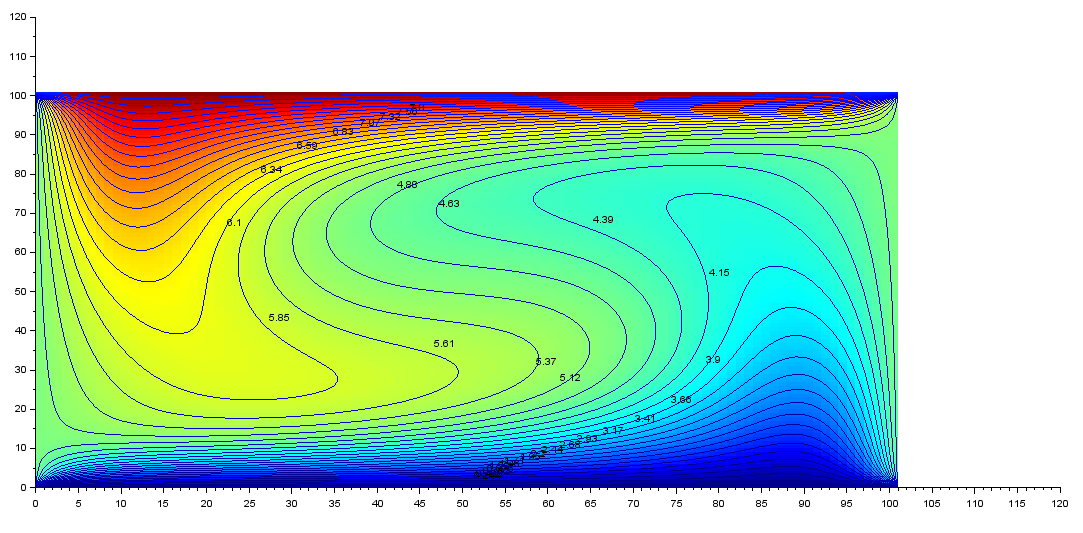
\includegraphics[width=\textwidth]{images/grafico_correto}

No entanto, para casos em que as dimensões da malha eram muito maiores que o número de iterações, ainda era possível ver pontos aleatórios no gráfico:

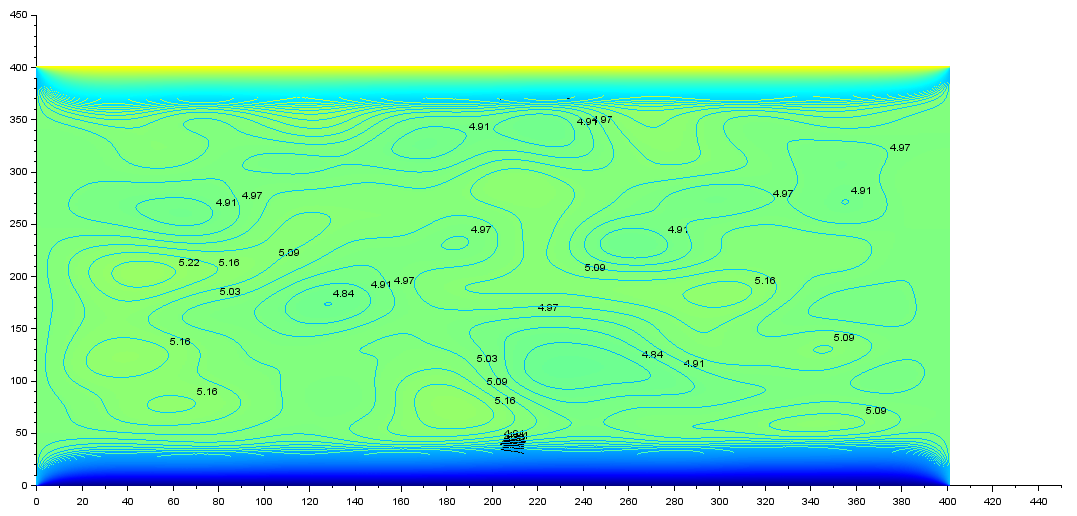
\includegraphics[width=\textwidth]{images/grafico_errado}

Este resultado é intuitivo, porque a cada iteração os valores das bordas influenciam cada vez mais os pontos internos da malha. Se o número de iterações é baixo em relação a dimensão da malha, não sobra tempo para os valores das bordas influenciarem o cálculo da solução dos pontos mais próximos do centro.

Em relação ao ganho de desempenho, podemos perceber pela planilha (\texttt{medidas.ods}) que a versão paralela supera a versão sequencial principalmente por conta do crescimento das dimensões da malha e do número de iterações. Outras variáveis, como o tamanho dos blocos, tiveram impacto mínimo no desempenho.

O maior ganho da versão paralela foi justamente com os maiores valores de $N_1, N_2$ e $iter$ testados, obtendo aceleração de $6.757473$ para uma malha $1000x1000$ e $5000$ iterações.

Também notamos que a sobre-relaxação sucessiva \textbf{local} provocou, consistentemente, tempos de execução maiores, se comparados com execuções com os mesmos parâmetros e sobre-relaxação sucessiva com $\omega$ fixo. Apesar disso, a sobre-relaxação sucessiva \textbf{local} também causou aceleração maior do algoritmo paralelo.

\end{document}
